\documentclass[11pt]{IEEEtran}
% correct bad hyphenation here
%\hyphenation{op-tical net-works semi-conduc-tor}

\usepackage{algorithm, algpseudocode, amsmath, cite, graphicx, multirow, url}

\makeatletter
\newcommand{\removelatexerror}{\let\@latex@error\@gobble}
\makeatother

\renewcommand\thesection{\arabic{section}}
\renewcommand\thesubsection{\thesection.\arabic{subsection}}
\renewcommand\thesubsubsection{\thesubsection.\arabic{subsubsection}}

\renewcommand\thesectiondis{\arabic{section}}
\renewcommand\thesubsectiondis{\thesectiondis.\arabic{subsection}}
\renewcommand\thesubsubsectiondis{\thesubsectiondis.\arabic{subsubsection}}

\begin{document}

\title{Tag Recommendations in StackOverflow}
\author{Logan~Short, Christopher~Wong, and~David~Zeng}% <-this % stops a space
\markboth{CS 224W Final Project, Autumn 2014}{}
\maketitle

\begin{abstract}
Abstract goes here.
\end{abstract}

\section{Introduction}

\IEEEPARstart{I}{n} many community-based information web sites, such as StackOverflow, users contribute content in the form of questions and answers, allowing others to learn through the collaboration and contributions of the community. These web sites often rely upon tags as metadata that assists in the indexing, categorization, and search for particular content with just a few key words. Almost always, users are given the responsibility to choose tags which identify their own content. Tagging, however, can prove to be a confusing process for inexperienced users who may not be familiar with the tags available to them. In addition, general human error or malicious users could lead to improperly tagged posts that disrupt the organization of information on the website.

As such, there is a clear motivation behind implementing stronger and more accurate tag recommendation systems. The most obvious benefit stems from the fact that tags help ensure that website data is properly categorized and thus easily searchable by users. A tag recommendation model can improve tag accuracy and effectiveness in a number of ways. For example, new users would not have to worry as much when choosing appropriate tags for their questions, and so the act of asking questions is an easier experience along with the better tags being chosen. Furthermore, recommending tags decreases the possibility of introducing \textit{tag synonyms} into the tagspace, as is commonly done through human error. Tag synonyms are discussed more in Section III.

The development of tag recommendation systems for user created content is a relatively new field and most previous work has taken place within the last couple of years. Thus, tag recommending is a field in which the state of the art is still being actively developed, and the most accurate methods for recommending tags have yet to be established. Software information web sites and other such services that are based on user produced content rely on the interactions between users and consequently are governed by an underlying network structure. It is thus probable that network structure could be used to assess user content and obtain accurate tag recommendations. Based on this intuition, the goal of our work is to analyze whether the underlying network structure of software information sites can be used to accurately recommend tags for user produced content and to potentially advance the state of the art in this still developing field.

\section{Prior Work}

Before analyzing existing implementations of tag recommendation systems, we found abundant relevant information regarding the growth and properties of groups and communities in large social networks. In \cite{2}, McAuley and Leskovec propose an algorithm to automatically discover social circles by analyzing the similarities among user profiles in data drawn from the social networking sites Facebook, Google+, and Twitter. Using the idea that nodes are well connected within a circle, the algorithm finds the best parameters to determine which edges should exist in an ego network. In \cite{3}, Backstrom et al. analyze the evolution of communities in social networks over time. The authors use a decision tree model to classify communities as fast- or slow-growing and show that connectedness of the community within and to those outside of the community plays a huge role in growth rate.

In \cite{1}, Xia et al. propose an automatic tag recommendation algorithm \textit{TagCombine}. There are three components of \textit{TagCombine}, each of which tries to assign the best tags to untagged objects: (1) multi-label ranking component, which predicts tags using a multi-label learning algorithm, (2) similarity based ranking component, which uses similar objects to recommend tags, and (3) tag-term based ranking component, which analyzes the historical affinity of tags to certain words in order to suggest tags. The recommendation algorithm methodically computes various weighted sums of the three components to attempt to find the best overall model. A $recall@k$ score is then calculated for each prediction model from stratified $10$-fold cross validation. (The $recall@k$ metric is discussed more in Section $4$.) The results demonstrate that \textit{TagCombine} performs significantly better than all other cited models.

In \cite{5}, Wang et al. propose a tag recommendation system dubbed \textit{EnTagRec}. The proposed \textit{EnTagRec} computes tag probability scores using two separate methods, Bayesian Inference and Frequentist Inference, and then takes a weighted sum of the probability scores. Bayesian Inference relies on a post’s textual data to compute the probability that a given tag is associated with the post. \textit{EnTagRec} formulates posts into a bag-of-words model and then trains a Labeled Latent Dirichlet Allocation model which is used to compute tag probability scores for a post. The Frequentist Inference approach infers a set of tags after some preprocessing of a post. Once this set is computed, \textit{EnTagRec} applies spreading activation to a tag network constructed by examining the co-occurrence rate of tags on the site. Experimental results show that \textit{EnTagRec} performs significantly better than \textit{TagCombine} from \cite{1} on Stack Overflow, Ask Ubuntu, and Ask Different datasets, but yields only comparable results on Freecode datasets.

In \cite{1}, Xia et al. propose a recommendation system that relates the textual features of posts to tags with reasonably good results. However, one weakeness of \textit{TagCombine} is that it fails to look at the network structure of software information sites. Posts on sites like Stack Overflow are ultimately connected to each other through an underlying network structure where users and tags that appear on multiple posts represent connections between said posts. In fact, the main purpose of tags is to group similar posts and create an organized structure that allows for more convenient and logical browsing of posts. Thus, it is not too farfetched to conjecture that knowledge of the network’s structure could be used to enhance a tag recommendation system. In \cite{5}, Wang et al. provide evidence that such an approach could yield significant improvement in tag recommendation results. In \cite{5}, the basic \textit{TagCombine} model proposed in \cite{1} is enhanced into a model that uses not only textual analysis of posts, but also network analysis of the tags themselves. Although results improved, the use of network structure is very limited, and further incorporation of network structure could potentially lead to more accurate tag recommendations.

One weakness in both \cite{1} and \cite{5} is that they both only address tag recommendations during question creation time. That is, tag recommendations need to be made with just the text from the initial post. Discussion generated over time by the post is not factored into the features for the tag recommendation system. However, tagging a post is not an action limited to post creation time.
Information contained in a post’s discussion could provide additional clues as to what the proper tags of the original question should have been, especially if the original question was poorly worded or unclear. In addition, users may add additional tags to posts later on based on the resulting discussion and evolution of the original question. In the context of a social network, this is similar to the notion of users joining new communities: posts can acquire new tags over time. Node clustering could also be used to potentially obtain accurate tag recommendations. In \cite{2}, McAuley and Leskovec discuss a method for automatically detecting ``circles'' in networks of users based on similarities in user profiles. A natural extension of this method would be to detect posts associated with common tags based on the similarities in features of the posts or to find circles of tags or users that could allow for accurate detection of possible associated tags using a given tag. Both situations are realistic for clustering tags, users, or posts on software information sites.

\section{Data and Network Analysis}

We begin by discussing our data collection and some key points in our preprocessing of the StackOverflow dataset in III.$A$ and III.$B$. We then explore various graphs that can be constructed from the underlying StackOverflow network structure, which we will apply in our new tag recommendation model.

\subsection{Data Collection}

StackOverflow is a member of the Stack Exchange network, and all user content contributed on this network is cc-by-sa 3.0 licensed. Our data set is the September 26, 2014 snapshot for StackOverflow, downloaded from the Stack Exchange data dump (see \cite{6}). The raw data set contains approximately 20 gigabytes (GB) of compressed XML files corresponding to Badges, Comments, PostHistory, PostLinks, Posts, Tags, Users, and Votes.

\subsection{Tag Synonyms}

We refer to two tags as tag synonyms if their names are different but they refer to the same concept, such as \texttt{.net-3.5} and \texttt{.net-framework-3.5}. Tag synonyms are a direct result of a question poster being given full discretion to assign tags to his or her post and to arbitrarily create new tags. This negatively impacts the strength of the tagspace, since a user searching for questions related to \texttt{.net-3.5} could completely miss the highly-related questions tagged with \texttt{.net-framework-3.5}. While we intend our tag recommendation system to help prevent future synonym groups, the currently existing groups must be addressed.  Since the pruning of tag synonyms is currently done manually by volunteer contributors, there are still many synonym groups throughout the site. Figure~\ref{fig:syn} is a screenshot of the \textit{Tag Synonyms} page of StackOverflow taken on December 9, and we can see that the maintenance of this list varies in consistency.\\

\begin{figure}[h]
  \centering
    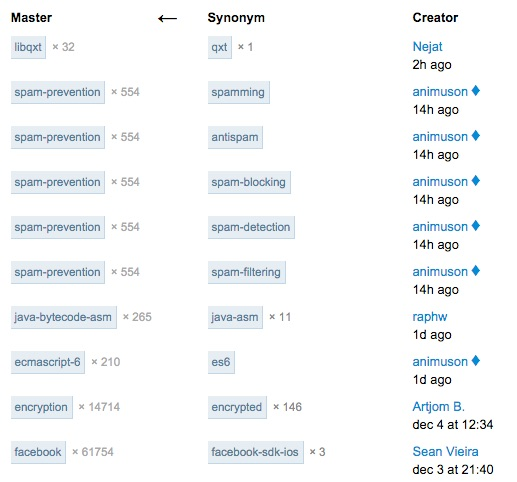
\includegraphics[width=3.2in]{tagsynonyms_so.jpg}
  \caption{Screenshot of \textit{Tag Synonyms} page.}
  \label{fig:syn}
\end{figure}

To be able to test the effects of tag synonyms on our tag recommendation model, we prepared a separate tag list derived from our initial set of $437$ after manually pruning for tag synonyms. Since these tags are among the more popular tags in the StackOverflow community, we were only able to reduce this new set to a size of $428$ after coalescing tags such as \texttt{report} and \texttt{reporting}. We expect this pruned list of tags to moderately, but not drastically, improve our results.

\subsection{Network Features}

The underlying structure of the StackOverflow network is diverse and complex since users and tags can be related through various questions, answers, and comments. We picked certain relationships between objects that we deemed to likely be the most indicative of the best tags to recommend and constructed the appropriate graphs. We briefly describe them in the following sections.

\subsubsection{Network Based on Post Similarity}

A natural graph to consider on the StackOverflow data would be the graph in which the nodes are questions and edges connect two questions if tf-idf vectors of their textual bodies have cosine similarity above a certain threshold. This graph essentially connects posts in StackOverflow based on a measure of topical similarity. The following plot shows the degree distribution of such a graph when the threshold for cosine similarity is chosen to be $0.3$.

\begin{figure}[h]
  \centering
    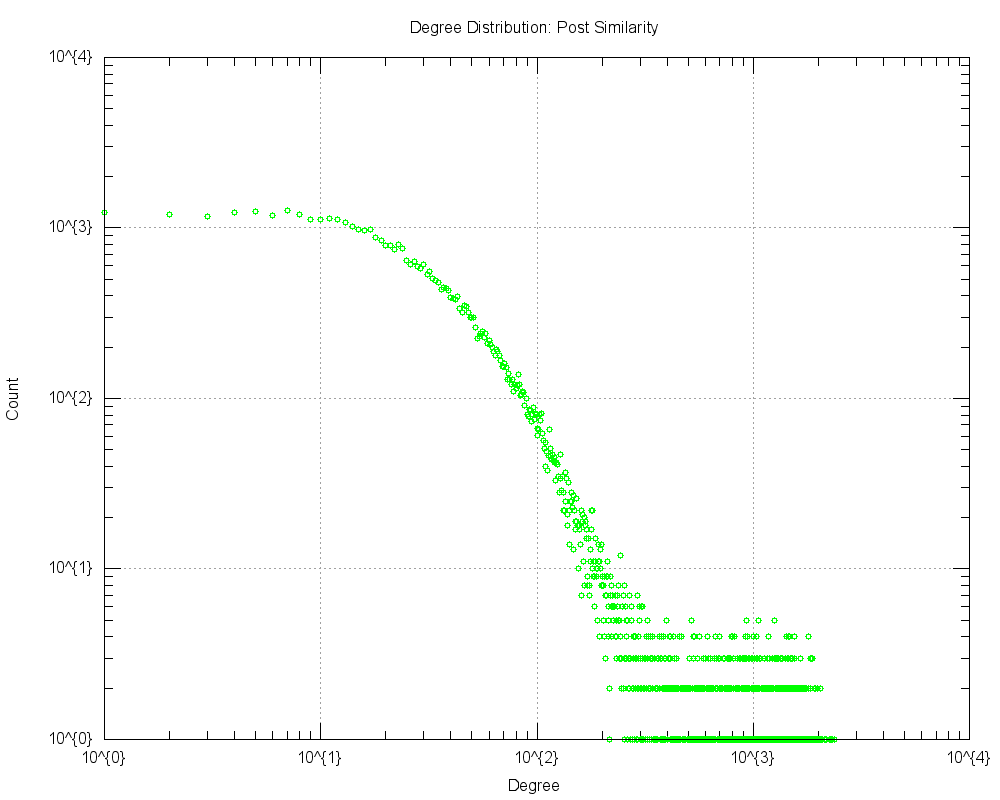
\includegraphics[width=3.2in]{similarity_degdistr.png}
  \caption{Degree distribution of the Post Similarity network.}
  \label{fig:post_dd}
\end{figure}

We notice that this degree distribution looks much like a power law distribution. Most questions are only similar to a few other questions on StackOverflow, while a few questions are similar to many others. In particular, we can observe the kinds of questions that are similar to many others. Here is one such question: http://stackoverflow.com/questions/121656/regular-expression-to-remove-xml-tags-and-their-content.
Notice that this post references XML parsing, C\#, .NET, and regular expressions, all of which are very common topics on StackOverflow. In general, the posts that have high degrees are at the intersection of multiple popular topics. This is backed up by \cite{8}, in which we see that the intersection of communities in a network are densely connected. These well-connected posts are likely to lie at the intersection of communities in this network, which motivates us to use this graph in tag recommendation. Since tags are StackOverflow’s method of organizing posts into topical categories or communities, extracting communities on this graph could lead to information about what tags to recommend to new questions that are similar to posts in a given community.

\subsubsection{Network Based on User Interaction}

We also experimented with the following StackOverflow network. The users of StackOverflow are represented as nodes of our network. Two users $u$ and $v$ are linked with an edge if $u$ answers a question posted by $v$ such that the answer reaches a predefined threshold in positive rating. In this case, two users share similar topical interests, which lead to their interactions on StackOverflow through question and answer. Below is a plot of the degree distribution of this network.

\begin{figure}[h]
  \centering
    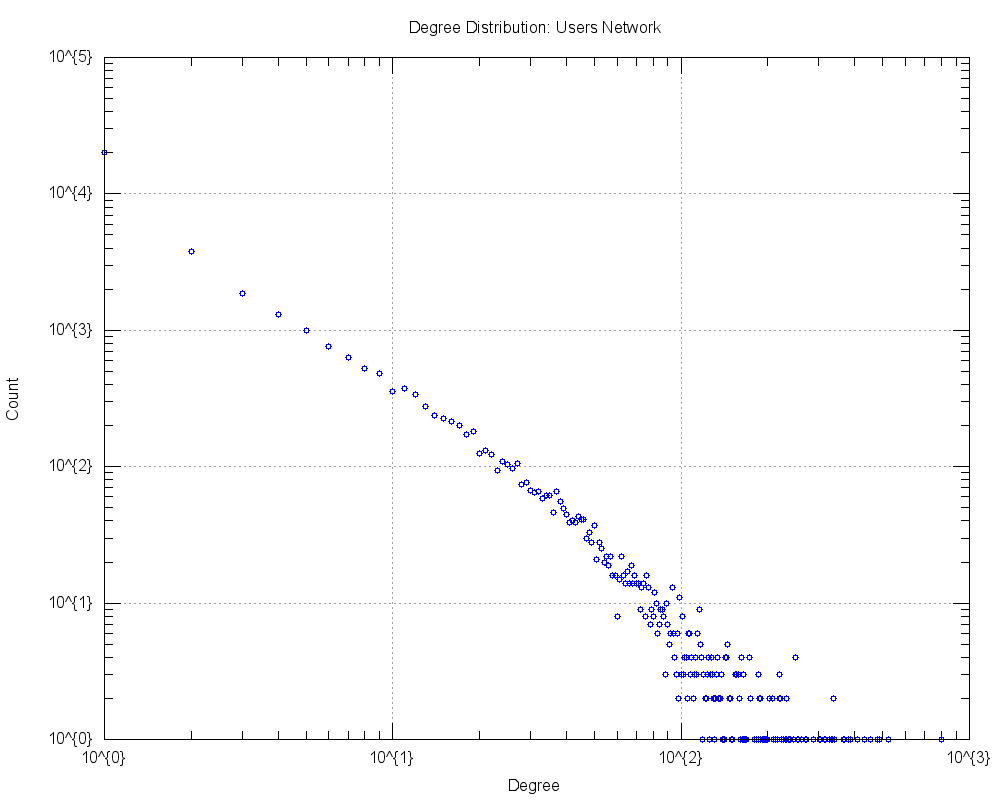
\includegraphics[width=3.2in]{user_degdistr.png}
  \caption{Degree distribution of the User Interaction network.}
  \label{fig:user_dd}
\end{figure}

The power law distribution occrus as a result of the following explanation. The users with degrees between $10$ and $100$ have the highest question to answer ratio, around $0.196$, while the users with degrees between $1$ and $10$ have the lowest question to answer ratio, around $0.118$. This means that a question posted on StackOverflow is likely to elicit multiple answers, resulting in a medium sized degree for users that post questions. Many infrequent users that answer questions will only receive interactions with the user that posted the question leading to low degrees for these users. On the extreme end, users with degree over $100$ have answered on average $148$ questions, which indicate that the tail of the distribution is populated mainly by power users or experts on StackOverflow.

The motivation for using such a graph banks on the assumption that users probably only post on a few topics in StackOverflow, and that new questions by a user are likely to share tags with a previous post. Thus, if we could organize users into communities and assign tag representatives for these communities, these tag representatives could become recommendations for questions posted by users from that community.


\subsubsection{Bipartite Graph between Users and Tags}

On sites such as Stack Overflow, relationships exist between users and tags since users will tend to interact most with the tags they are interested in or posses the most expertise with. In order to analyze these relationships we generated a bipartite graph where nodes on one side of the graph represented users and nodes on the opposite side of the graph represented tags. The edges of the graph were constructed and weighted to represent a user’s contribution and interaction with each tag. Questions, answers, and comments made by a user on a post associated with a particular tag each contributed to that user’s score with the tag in question. User made questions were evaluated as the most significant form of contribution to a tag since each post is defined by the original question and thus added the most to a user’s tag score. Answers were evaluated as the next most significant form of contribution since answers make up the majority of the structure of a post not including the question and require some level of expertise with the tags associated with the post. Comments were evaluated as significantly less indicative of a contribution to a tag since they are generally not a significant contribution to the content of a post. User tag scores were then used as weights for the edges connecting each user to each tag. Tags which scored 0 points with a user did not contain an edge to that user since this meant that the user had not interacted with the tag. Below is a plot of the degree distribution of the users in the bipartite graph.

\begin{figure}[h]
  \centering
    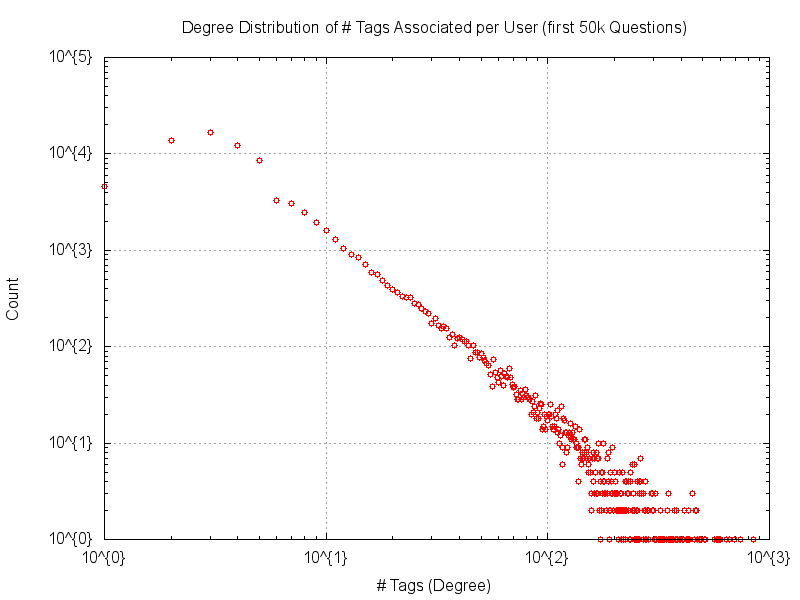
\includegraphics[width=3.2in]{bipartite_degdistr.png}
  \caption{Degree distribution of the bipartite graph between users and tags.}
  \label{fig:bi_dd}
\end{figure}

From the plot we can see that the number of tags each user was associated with followed a power law distribution. This indicates that most users interact with a very small number of tags while a select few users contribute to a large number of tags. Such a trend is consistent across many social networks with the vast majority of users having a very limited number of connections and only a small portion of users having a large amount of connections. Thus the degree distribution suggests that the users on Stack Overflow behave in a manner similar to those of other social networks. In addition, the fact that most users are associated with a limited pool of tags suggests that recommending tags based on users associated with a post could yield accurate results. For example, if the majority of users interacting on a post all have high tag scores with the same tag, then since most users have a limited pool of associated tags we can be confident that the post in question should be assigned the shared tag.

\section{Algorithm and Results}

\subsection{Original TagCombine Components}

To begin, using the procedures described in \cite{1}, we implemented the three major components of the \textit{TagCombine} algorithm to establish a baseline for the performance of our tag recommendation system. By reproducing a working implementation of \textit{TagCombine}, we were able analyze the effect of our improvements on tag recommendation accuracy.

As alluded to earlier, \cite{1} introduces the concept of the $recall@k$ metric for measuring the success of a tag recommendation model, where $k$ is a tunable parameter that determines how many tags the model recommends for each object. Intuitively, over $n$ objects, the $recall@k$ metric measures the average success rate in predicting correct tags for each object, where a ``correct'' tag is simply a tag that has been used to label that particular object by an actual user. Let $R_i$ be the set of tags recommended for object $i$ (so, $|R_i| = k$), and let $T_i$ be the actual set of tags used to label object $i$. Then, the formula for $recall@k$ is:

\[recall@k = \frac{1}{n}\sum\limits_{i=1}^{n}\frac{|R_i \cap T_i|}{|T_i|}.\]

\subsubsection{Multilabel Learning Algorithm}

\subsubsection{Similarity Based Ranking Component}

The second component of \textit{TagCombine} is based on assigning tags based on similar posts. Given a new question $q$, \textit{TagCombine} first finds similar posts to $q$ using cosine similarity. First the idf of each term in our dictionary is computed. The idf of a term $t$ is given by the formula
\[ \text{idf}(t) = \frac{\# \text{ of total documents}}{\log (\# \text{ of documents containing t} )} \]
Next, for all posts $p$, the tf-idf of a term $t$ in a post $p$ is computed using
\[ \text{tfidf}(t,p) \mathbf{tf}(t, p) \times \mathbf{idf}(t)\]
where $\mathbf{tf}(t, p)$ is the raw frequency of the term $t$ in post $p$. The tf-idf vector of a post $p$, $\text{tfidf}(p)$, then refers to the vector of $\text{tfidf}(t,p)$ values over all terms $t$. The cosine similarity between an old post $p$ and the new question $q$ would therefore be
\[ \text{sim}(p, q) = \frac{\text{tfidf}(p) \times \text{tfidf}(q)}{\|p\| \|q\|}.\]
Using this cosine similarity formula, we can find $p_1, \ldots, p_{50}$, the $50$ most similar posts to $q$. Let $T_1, \ldots, T_{50}$ denote the sets of tags used in each of these posts. We compute a likelihood for each tag $g$ for question $q$ using the following formula
\[ L(g, q) = \frac{ |\{i : g \in T_i \} | }{\sum_i  |T_i |}\]


\subsubsection{Tag-term Based Ranking Component}

\subsubsection{Analysis of TagCombine}

\subsection{New Network Based Ranking Component}

\subsubsection{Modification to Similarity Component}

\subsection{NetTagCombine Algorithm}

In our proposed tag recommendation system, \textit{NetTagCombine}, we add our new Network-Based Ranking Component, alongside the other components of \textit{TagCombine}. Building upon the equation for \textit{TagCombine} given in \cite{1}, for all tags $t$ with respect to some post $p$, our new \textit{NetTagCombine} score can be given by
\begin{align*}
NetTagCombine_p(t) =\ &\alpha \times MultiLabel_p(t) +\\
&\beta \times SimRank_p(t) +\\
&\gamma \times TagTerm_p(t) +\\
&\delta \times Network_p(t)
\end{align*}
where $\alpha,\beta,\gamma,\delta \in [0,1]$ represent the different weights of the components. Here, we have added the term of $\delta \times Network_p(t)$ to represent our new fourth component that uses the underlying network structure. To adjust for this fourth component, here is the pseudocode for \textit{NetTagCombine}:


\begin{algorithm*}
  \caption{\textit{NetTagCombine} algorithm}\label{ntc}
  \begin{algorithmic}[1]
    \State $\alpha, \beta, \gamma, \delta \gets 0$
    \For{\textbf{all }posts $p$}
      \For{\textbf{all }tags $t \in TAGS$}
        \State Compute \textit{MultiLabel}$_p(t)$, \textit{SimRank}$_p(t)$, \textit{TagTerm}$_p(t)$, and \textit{Network$_p(t)$}
      \EndFor
    \EndFor
    \For{\textbf{all }$\alpha$ from $0$ to $1$, every time increment by $0.2$}
      \For{\textbf{all }$\beta$ from $0$ to $1$, every time increment by $0.2$}
        \For{\textbf{all }$\gamma$ from $0$ to $1$, every time increment by $0.2$}
          \For{\textbf{all }$\delta$ from $0$ to $1$, every time increment by $0.2$}
            \State Compute \textit{NetTagCombine}$_p(t)$ for all tags $t$ on posts $p$
            \State Evaluate effectiveness of $(\alpha,\beta,\gamma,\delta)$ from $recall@k$ scores
          \EndFor
        \EndFor
      \EndFor
    \EndFor\\
    \Return Best $(\alpha,\beta,\gamma,\delta)$\;
  \end{algorithmic}
\end{algorithm*}

\subsection{Results}

\section{Conclusion}

\subsection{Future Work}

\begin{thebibliography}{1}
\bibitem{1} X. Xia, D. Lo, X. Wang, B. Zhou. Tag Recommendation in Software Information Sites. MSR, 2013.
\bibitem{2} J. McAuley, J. Leskovec. Discovering Social Circles In Ego Networks. ACM TKDD, 2014.
\bibitem{3} L. Backstrom, D. Huttenlocher, J. Kleinberg, X. Lan. Group Formation in Large Social Networks: Membership, Growth, and Evolution. KDD, 2006.
\bibitem{4} J. Leskovec, K. Lang, A. Dasgupta, M. Mahoney. Statistical Properties of Community Structure in Large Social and Information Networks. WWW, 2008.
\bibitem{5} S. Wang, D. Lo, B. Vasilescu, A. Serebrenik. EnTagRec: An Enhanced Tag Recommendation System for Software Information Sites. ICSME, 2014.
\bibitem{6} Stack Exchange Data Dump (September 26, 2014). Retrieved 2 November 2014. https://archive.org/details/stackexchange.
\bibitem{7} Overlapping Community Detection at Scale: A Nonnegative Matrix Factorization Approach. WSDM, 2013.
\bibitem{8} Community-Affiliation Graph Model for Overlapping Network Community Detection. ICDM, 2012.
\end{thebibliography}

\appendix

Hi

%\balancecolumns

\end{document}
